\documentclass{article}

\usepackage{array}
\usepackage{graphicx}

\begin{document}

\title{Week 7, Session 2 Problems}
\author{GSI: Caleb Eades}
\date{10/4}
\maketitle

\section{Finding Electric Fields}

\subsection{Progressive Derivations}

(Note: this is the last problem from Week 7, Session 1 Problems in case you didn't get around to it. It is a good problem to know.)

This problem asks you to find the electric field from progressively more complex charge distributions. Indeed, part (c) seems very hard to solve for. [Hint: use the result of part (a) for part (b). Similarly, use the result of part (b) for part (c).]
\begin{itemize}
	\item[(a)] Suppose there is a ring of charge of radius $r$ centered at the origin in the xy-plane with linear charge density $\lambda$. Calculate the field at a point $P$ that is at $(x,y,z)=(0,0,d)$.
	\item[(b)] Suppose there is a disk of radius $R$ centered at the origin in the xy-plane with area charge density $\sigma$. Calculate the field at the same point $P$.
	\item[(c)] Suppose there is a a cylinder of radius $R$ centered at the origin in the xy-plane with its bottom surface in that plane, extending a height $h$ upwards along its axis, the z-axis. If this cylinder has charge density $\rho$, calculate the field at the same point $P$, assuming $h<d$.
\end{itemize}

\section{Previous Midterm Problems}

\subsection{Non-Uniform Charge Distributions?!}

A non-uniformly charged ring of radius $R$ carries a linear charge density $\lambda$($\theta$)$=\lambda_0$cos($\theta$), with $\lambda_0>0$. The ring lies in the ($x,y$) plane centered at the origin.
\begin{itemize}
	\item[(a)] Determine the direction of the electric field created at ($0,0,z$), and explain your reasoning.
	\item[(b)] Calculate the magnitude of the field.
	\item[(c)] A similar ring of linear charge density $\lambda$($\theta$)$=-\lambda_0$cos($\theta$) is placed at distance $2R$ from the first one along the symmetry axis. Determine the new field on the symmetry axis.
	\item[(d)] Make a qualitative plot of the magnitude on axis of the electric field between the two rings.
\end{itemize}

(\textit{Source: Bordel Spring 2013 Midterm 2})

\begin{figure}[h]
	\centering
	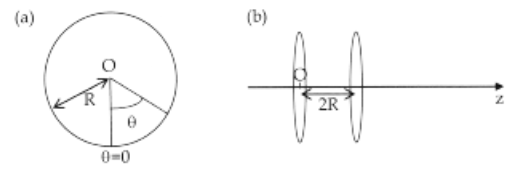
\includegraphics[width=0.6\textwidth]{BordelProblem.png}
	\caption{Setup for problem 2.1}
	\label{Bordel}
\end{figure}

\subsection{Fields from Rings}

A flat ring of inner radius $R_1$ and outer radius $R_2$ carries a non-uniform surface charge density $\sigma$($r$)$=\frac{\beta}{r}$, where $\beta$ is a positive constant, and $r$ is the radial distance measured form the center of the ring. Calculate the electric field produced by such a charge distribution at any point on the symmetry axis.

(\textit{Source: Bordel Spring 2014 Midterm 2})

\subsection{Dipoles with Lines}

Figure~\ref{Spelio} shows two equal and opposite charges, $q$, separated by a fixed distance, $d$. The rod connecting the two charges is at an angle, $\theta$, from the horizontal axis, and at a distance $r>>d$, form an infinite line of charge with charge per unit length, $\lambda>0$. \textit{\textbf{This line of charge points out of the page.}} Find the force $\vec{F}$, on the charges to the lowest, nontrivial order in $d/r$ when $\theta=0$ and when $\theta=90^o$. Express them in terms of any of the variables given and $\epsilon_0$.

(\textit{Source: Speliotopoulos Spring 2014 Midterm 2})

\begin{figure}[h]
	\centering
	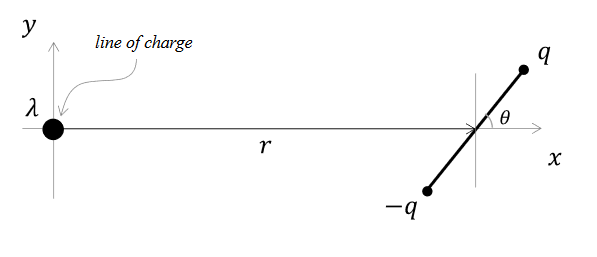
\includegraphics[width=0.6\textwidth]{SpelioProblem.png}
	\caption{Setup for problem 2.3}
	\label{Spelio}
\end{figure}

\end{document}